\documentclass[11pt]{article}
\usepackage[a4paper,margin=2cm]{geometry}
\usepackage{graphicx,booktabs,amsmath,float,caption,multirow}
\usepackage[hidelinks]{hyperref}
\setlength{\parskip}{4pt}\setlength{\parindent}{0pt}

\title{\textbf{PRML Lab 6 --- Dimensionality Reduction (PCA \& LDA)}}
\author{Aryan Tiwari (B20AI056)\\CSL2050 Pattern Recognition \& Machine Learning, Winter 2022}
\date{}

\begin{document}
\maketitle

\section*{Question 1 --- Principal Component Analysis}

\textbf{1. Reading the data and EDA.} \texttt{anneal.data} (798 rows) and \texttt{anneal.test} (100 rows) were parsed with the
38 attribute names from \texttt{anneal.names} and saved together as \texttt{data/anneal\_combined.csv}. Three things matter:
\begin{itemize}\itemsep0pt
\item \textbf{Severe class imbalance} --- class 3 is 76\% of the data, class 1 has only 8 samples and class 4 never occurs. Accuracy alone
would flatter a model that ignores the small classes, so I also report \textbf{macro-F1} and \textbf{balanced accuracy}.
\item \textbf{`?' mostly means ``not applicable'', not ``missing''} (as the dataset notes say). For most process flags the only values are a code or
`?', and 8 columns are over 99\% `?'. Imputing would invent data that does not exist, so `?' is kept as its own category, \texttt{NA}.
\item The numeric features have very different scales (thickness $\approx 1$, length up to 4880), so standardisation is essential before PCA.
\end{itemize}

\begin{figure}[H]\centering
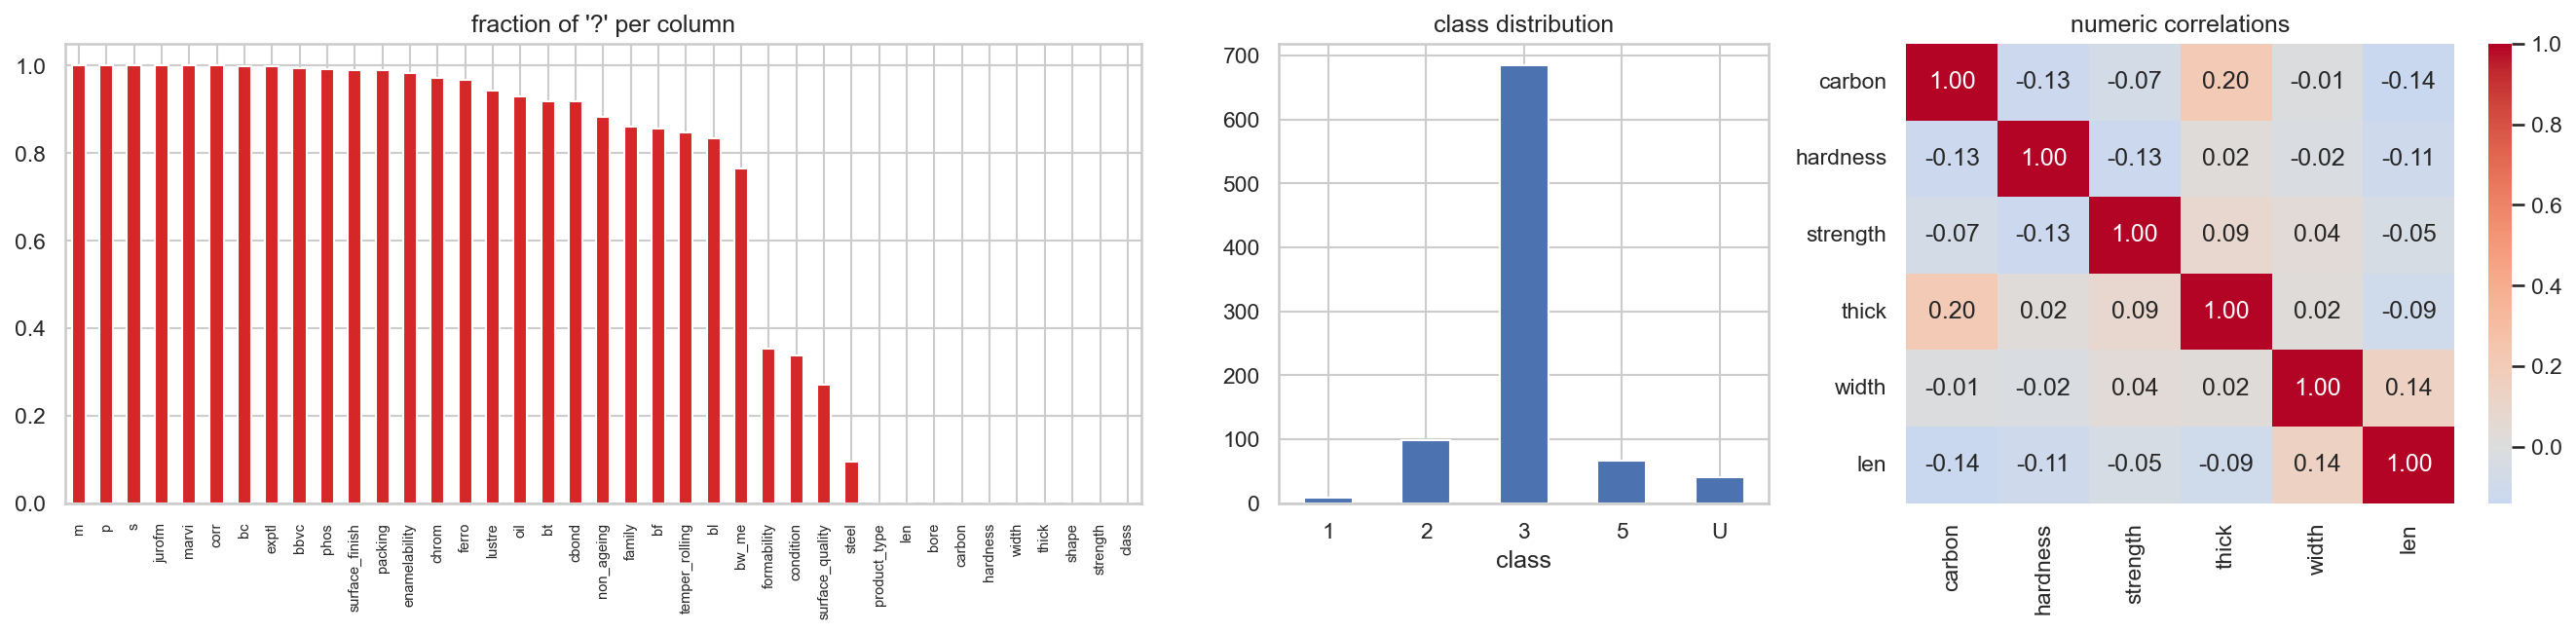
\includegraphics[width=\linewidth]{figures/q1_eda.png}
\caption{Share of `?' per column, class distribution, and correlations between the six numeric features.}
\end{figure}

\textbf{2. Pre-processing and split.} Twelve rows are exact duplicates; four of the \texttt{anneal.test} rows also appear in \texttt{anneal.data},
so both files were merged and de-duplicated (886 rows) before splitting, which prevents test rows from leaking into training. Seven
columns have a single value throughout and were dropped. The remaining 25 categorical columns were one-hot encoded, giving a 77-dimensional design matrix.
Split \textbf{65:35, stratified} (575 / 311), so that even class 1 appears in both parts. Every feature was standardised with the training mean and standard deviation.

\textbf{3. Classifiers and 5-fold CV.} \emph{Logistic regression} is a regularised linear baseline that suits one-hot data; \emph{KNN} ($k=5$)
depends entirely on distances, so it is the model most sensitive to PCA; a \emph{random forest} handles mixed features and
interactions without any tuning. Class weights are balanced where the model supports it.

\begin{figure}[H]\centering
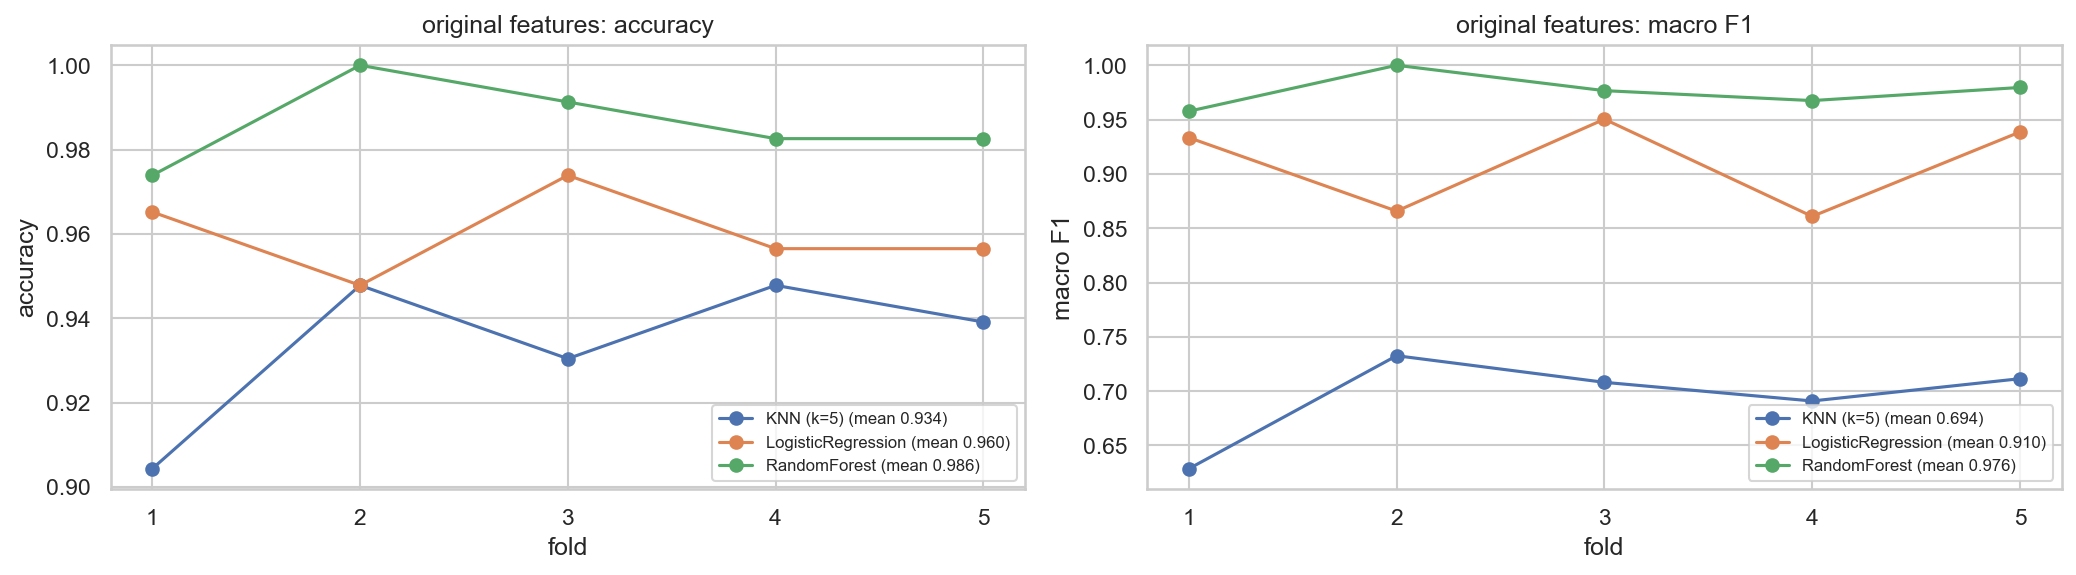
\includegraphics[width=\linewidth]{figures/q1_cv_original.png}
\caption{5-fold CV on the original 77 features.}
\end{figure}

\textbf{4. PCA from scratch.} (a) After standardisation the covariance matrix is computed as $\Sigma = X^\top X/(n-1)$.
(b) For a symmetric positive semi-definite matrix the SVD and the eigen-decomposition coincide ($\Sigma=V\Lambda V^\top$), so
\texttt{Singular\_Value\_Decomp} implements the \textbf{cyclic Jacobi eigenvalue algorithm}. It repeatedly applies plane rotations that
zero one off-diagonal pair at a time, until the off-diagonal mass is below $10^{-12}$; the accumulated rotations are the eigenvectors.
It converged in 8 sweeps on the $77\times77$ matrix. The eigenvalues match NumPy to $10^{-13}$ and $VV^\top = I$ to $10^{-14}$.
The principal components are $XV$.

\textbf{7. Choosing the number of components.} The variance is spread out: PC1 explains only 9.9\% and PC2 7.6\%, because one-hot
columns are only weakly correlated with each other. 90\%, 95\% and 99\% of the variance need 31, 36 and 44 components respectively. I used \textbf{$k=36$ (95\%)}.
The validation curve agrees: logistic regression keeps improving up to about 40 components, while the forest peaks
early ($k\approx 20$, macro-F1 0.863), because its trees work best on the original sparse columns.

\begin{figure}[H]\centering
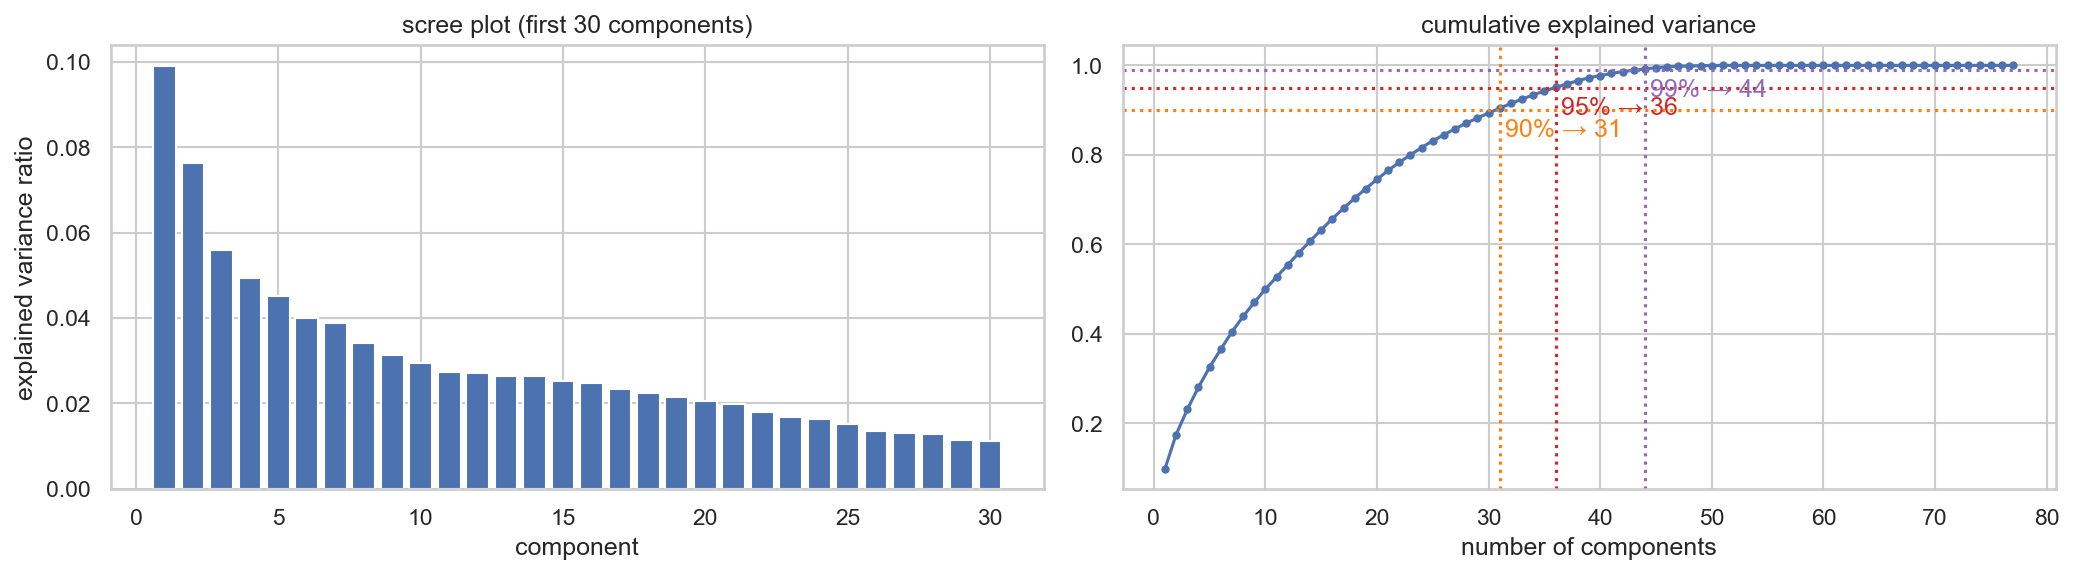
\includegraphics[width=\linewidth]{figures/q1_variance.png}\\
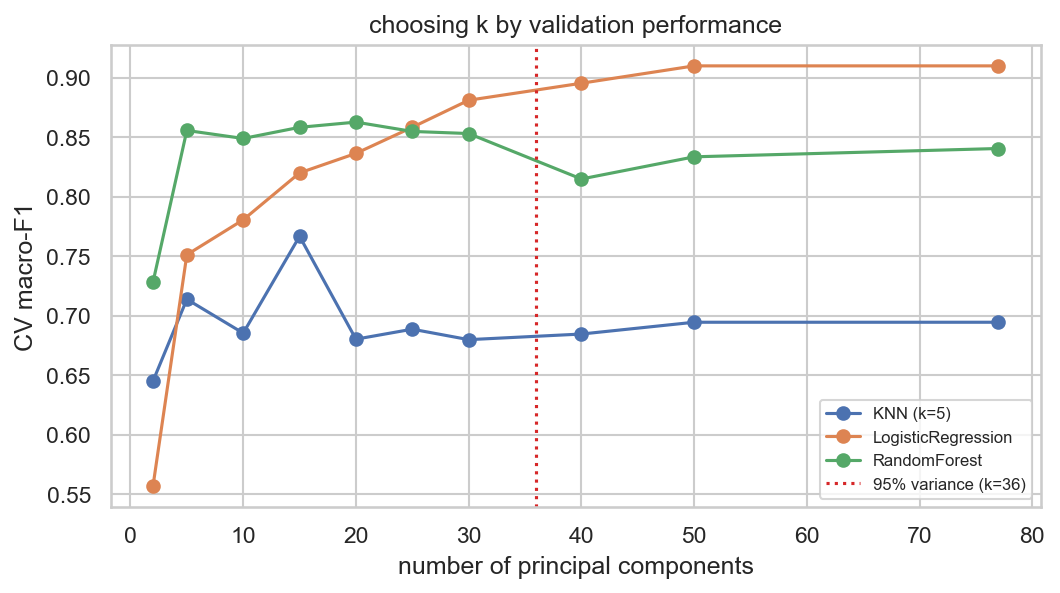
\includegraphics[width=0.6\linewidth]{figures/q1_k_selection.png}
\caption{Scree plot and cumulative variance (top); CV macro-F1 against the number of components (bottom).}
\end{figure}

\textbf{5--6. Results before and after PCA.}
\begin{table}[H]\centering
\begin{tabular}{llcccc}\toprule
Model & Features & CV macro-F1 & Test accuracy & Test balanced acc. & Test macro-F1\\\midrule
\multirow{2}{*}{Logistic regression} & original (77) & 0.910 & 0.965 & 0.925 & 0.911\\
 & PCA (36) & 0.882 & 0.929 & 0.916 & 0.840\\\midrule
\multirow{2}{*}{KNN ($k=5$)} & original (77) & 0.694 & 0.933 & 0.711 & 0.699\\
 & PCA (36) & 0.674 & 0.920 & 0.692 & 0.687\\\midrule
\multirow{2}{*}{Random forest} & original (77) & \textbf{0.976} & \textbf{0.990} & 0.913 & \textbf{0.948}\\
 & PCA (36) & 0.859 & 0.965 & 0.829 & 0.885\\\bottomrule
\end{tabular}
\end{table}
\textbf{PCA hurt every model here}, most of all the random forest (macro-F1 0.948 $\to$ 0.885). The 5\% of variance that PCA throws away is
not noise. For example, \texttt{family=TN} alone identifies class 5 perfectly, but it is a rare column with little variance, so PCA
mixes it into many components. The forest is hurt most because it relies on clean single-feature thresholds, and every PC mixes all
77 columns. Accuracy hides most of this damage because class 3 dominates; macro-F1 and balanced accuracy show it. KNN is
weak on the small classes either way, since with $k=5$ a class-1 point's neighbours are mostly class 3.

\textbf{7. Did the distribution change?} Yes. The PCs are exactly uncorrelated (largest $|r|$ between components $=10^{-14}$, compared with an average $|r|=0.09$
between the original features), the variance is concentrated in the leading directions, and the 36 kept PCs carry 73.3 of the 77.1 total units of
variance. In the PC1--PC2 plane class 5 already forms a separate cluster, but the other classes overlap, because PCA never looks at the labels.

\begin{figure}[H]\centering
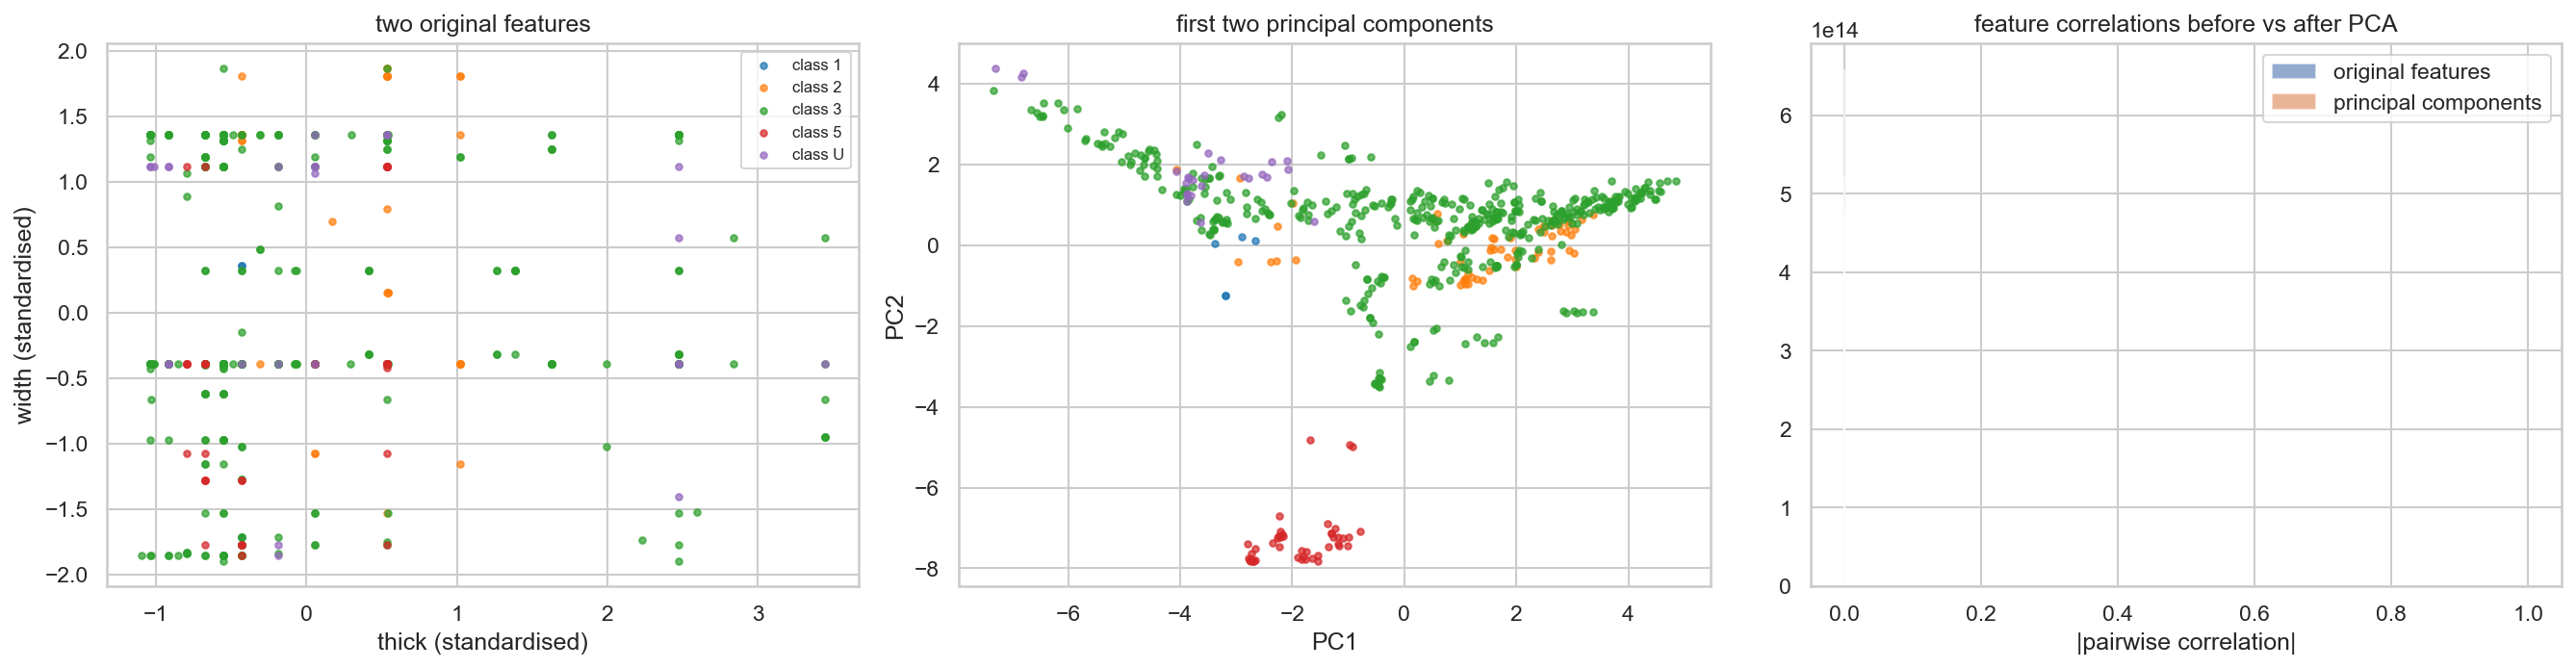
\includegraphics[width=\linewidth]{figures/q1_distribution.png}
\caption{Two original features vs.\ the first two PCs, and pairwise correlations before and after PCA.}
\end{figure}

\section*{Question 2 --- Linear Discriminant Analysis}

\textbf{1. LDA from scratch.} (a) The within-class scatter is $S_W=\sum_c\sum_{x\in c}(x-\mu_c)(x-\mu_c)^\top$ and the between-class scatter is
$S_B=\sum_c n_c(\mu_c-\mu)(\mu_c-\mu)^\top$. The discriminants are the leading eigenvectors of $S_W^{-1}S_B$. The one-hot columns of each
variable sum to one, so $S_W$ is singular; a small ridge ($10^{-3}\times$ the mean diagonal) is added, and the problem is solved in the
symmetric form $S_W^{-1/2}S_BS_W^{-1/2}$ using the same Jacobi routine.
(b) At most $C-1=4$ discriminants exist. The function keeps the smallest number whose eigenvalues reach a requested share:

\begin{table}[H]\centering
\begin{tabular}{lcccc}\toprule
 & LD1 & LD2 & LD3 & LD4\\\midrule
Eigenvalue & 1586.8 & 15.29 & 7.81 & 1.26\\
Share & 98.49\% & 0.95\% & 0.48\% & 0.08\%\\\bottomrule
\end{tabular}
\end{table}
Keeping 80\%, 90\% or 95\% selects 1 discriminant; keeping 99\% selects 2. LD1 is so dominant because \texttt{family=TN} occurs \emph{only
and always} in class 5 (all 67 samples). In that direction class 5 is perfectly separated with zero within-class spread, so the
between/within ratio becomes very large.

\textbf{2--3. PCA vs.\ LDA, and the features that matter most.}
\begin{figure}[H]\centering
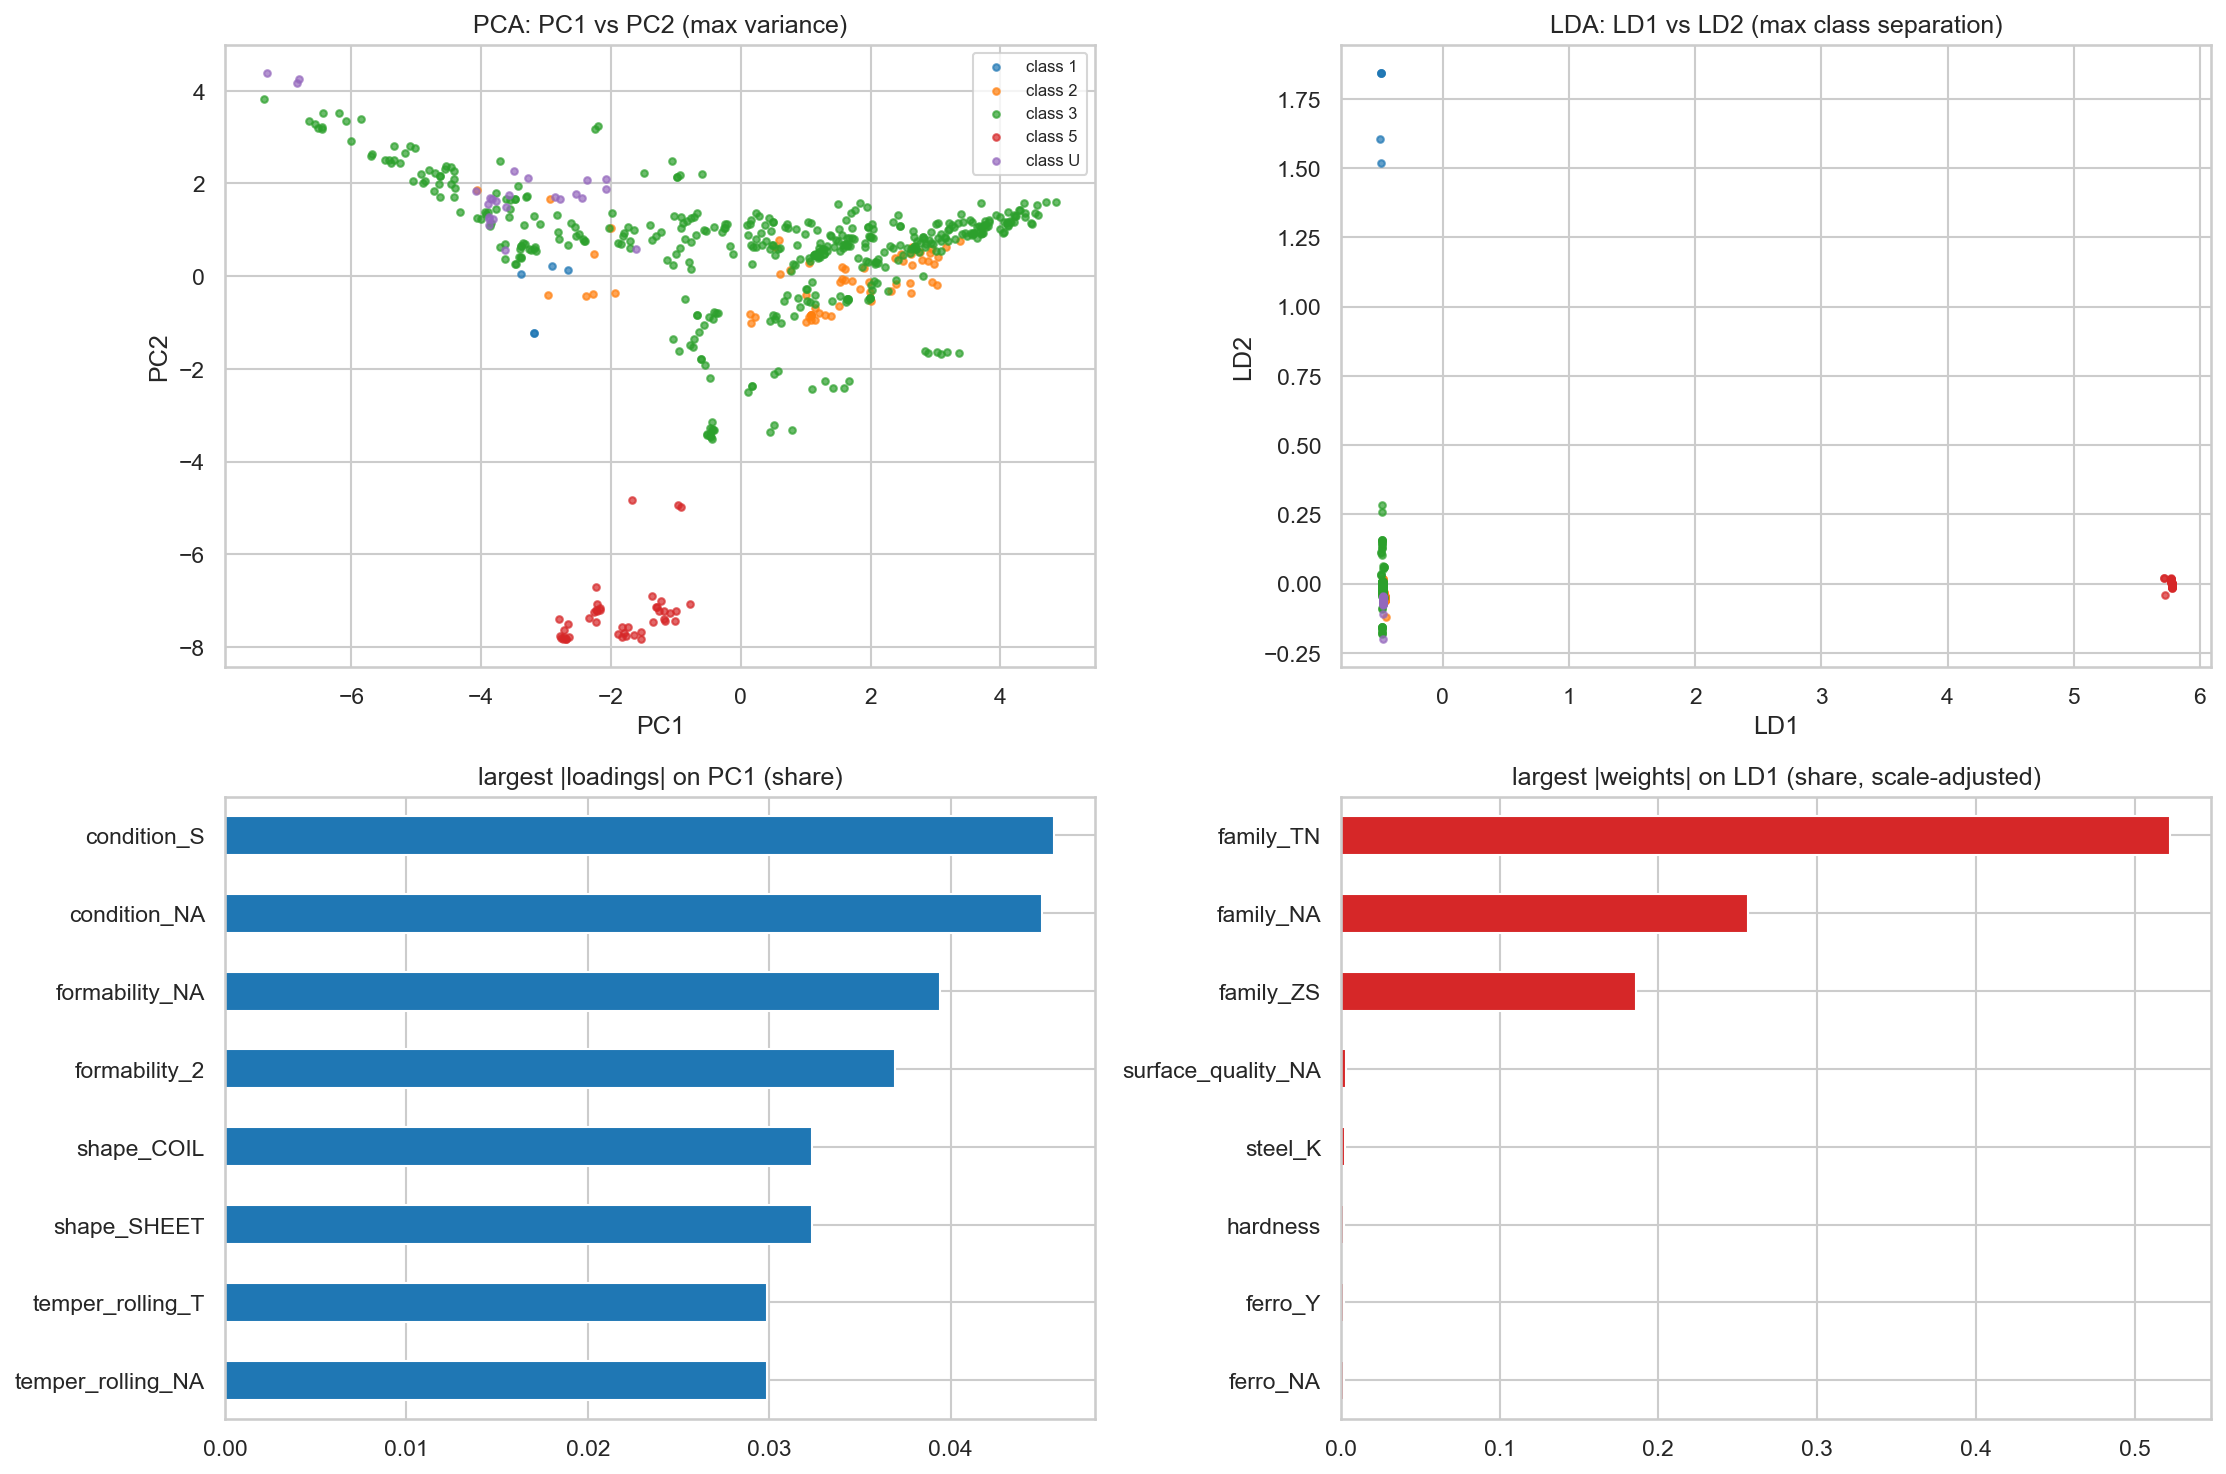
\includegraphics[width=0.95\linewidth]{figures/q2_pca_vs_lda.png}
\caption{Sample space in the first two PCs vs.\ the first two LDs (top), and the features with the largest weights (bottom).}
\end{figure}
PCA looks for directions of \emph{variance}. PC1 is spread across many process variables (condition, formability, shape, temper
rolling), each contributing only 3--5\%: these columns vary together across the whole dataset, whatever the class. LDA looks for directions of
\emph{class separation}. LD1 is almost entirely the \texttt{family} variable (TN 52\%, NA 26\%, ZS 19\%), which on its own splits off class
5, and LD2 isolates the tiny class 1. In the plots, classes 2, 3 and U overlap in the PCA plane, while in the LDA plane class 5 is
far to the right and class 1 is far above the rest, with only three dimensions left to separate classes 2, 3 and U.

\textbf{4. Feature extraction $\times$ classifier (test accuracy, both reduced to 4 dimensions).}
\begin{table}[H]\centering
\begin{tabular}{lcc}\toprule
 & KNN ($k=5$) & Logistic regression\\\midrule
PCA (4 PCs) & 0.942 \; (macro-F1 0.720) & 0.797 \; (macro-F1 0.653)\\
LDA (4 LDs) & \textbf{0.994} \; (macro-F1 \textbf{0.952}) & 0.929 \; (macro-F1 0.870)\\\bottomrule
\end{tabular}
\end{table}
At the same dimension LDA beats PCA with both classifiers, by 5 and 13 points of accuracy and 22--23 points of macro-F1.
The four LDA directions were chosen to separate the classes, while four PCs keep only 28\% of the variance and none of it is chosen
for its relevance to the classes. KNN on 4 LDs even beats every model on the full 77 features (99.4\%), because in LDA space distances
reflect class membership directly. Logistic regression gains less, because the LD space is already almost linearly separable and its
remaining errors are in the overlapping classes 2/3/U.

\textbf{5. LDA as a classifier --- 5-fold ROC/AUC from scratch.} The LDA classifier (shrinkage solver, because $S_W$ is singular) gives class
probabilities. ROC curves are computed one-vs-rest: the scores are sorted, TPR/FPR are counted at every distinct threshold, and the
area is integrated with the trapezoidal rule. The scratch micro-AUC for fold 5 (0.997561) matches \texttt{sklearn.metrics.roc\_auc\_score} exactly.

\begin{table}[H]\centering\small
\begin{tabular}{lcccccccc}\toprule
Fold & Accuracy & Micro AUC & Macro AUC & class 1 & class 2 & class 3 & class 5 & class U\\\midrule
1 & 0.930 & 0.995 & 0.965 & 1.000 & 0.998 & 0.961 & 1.000 & 0.866\\
2 & 0.957 & 0.993 & 0.997 & 0.996 & 1.000 & 0.991 & 1.000 & 1.000\\
3 & 0.974 & 0.999 & 0.998 & 1.000 & 1.000 & 0.997 & 1.000 & 0.993\\
4 & 0.983 & 1.000 & 1.000 & 1.000 & 1.000 & 1.000 & 1.000 & 1.000\\
5 & 0.939 & 0.998 & 0.997 & 1.000 & 0.997 & 0.988 & 1.000 & 0.998\\\midrule
Mean & 0.957 & \textbf{0.997} & \textbf{0.991} & 0.999 & 0.999 & 0.987 & 1.000 & 0.971\\\bottomrule
\end{tabular}
\end{table}

\begin{figure}[H]\centering
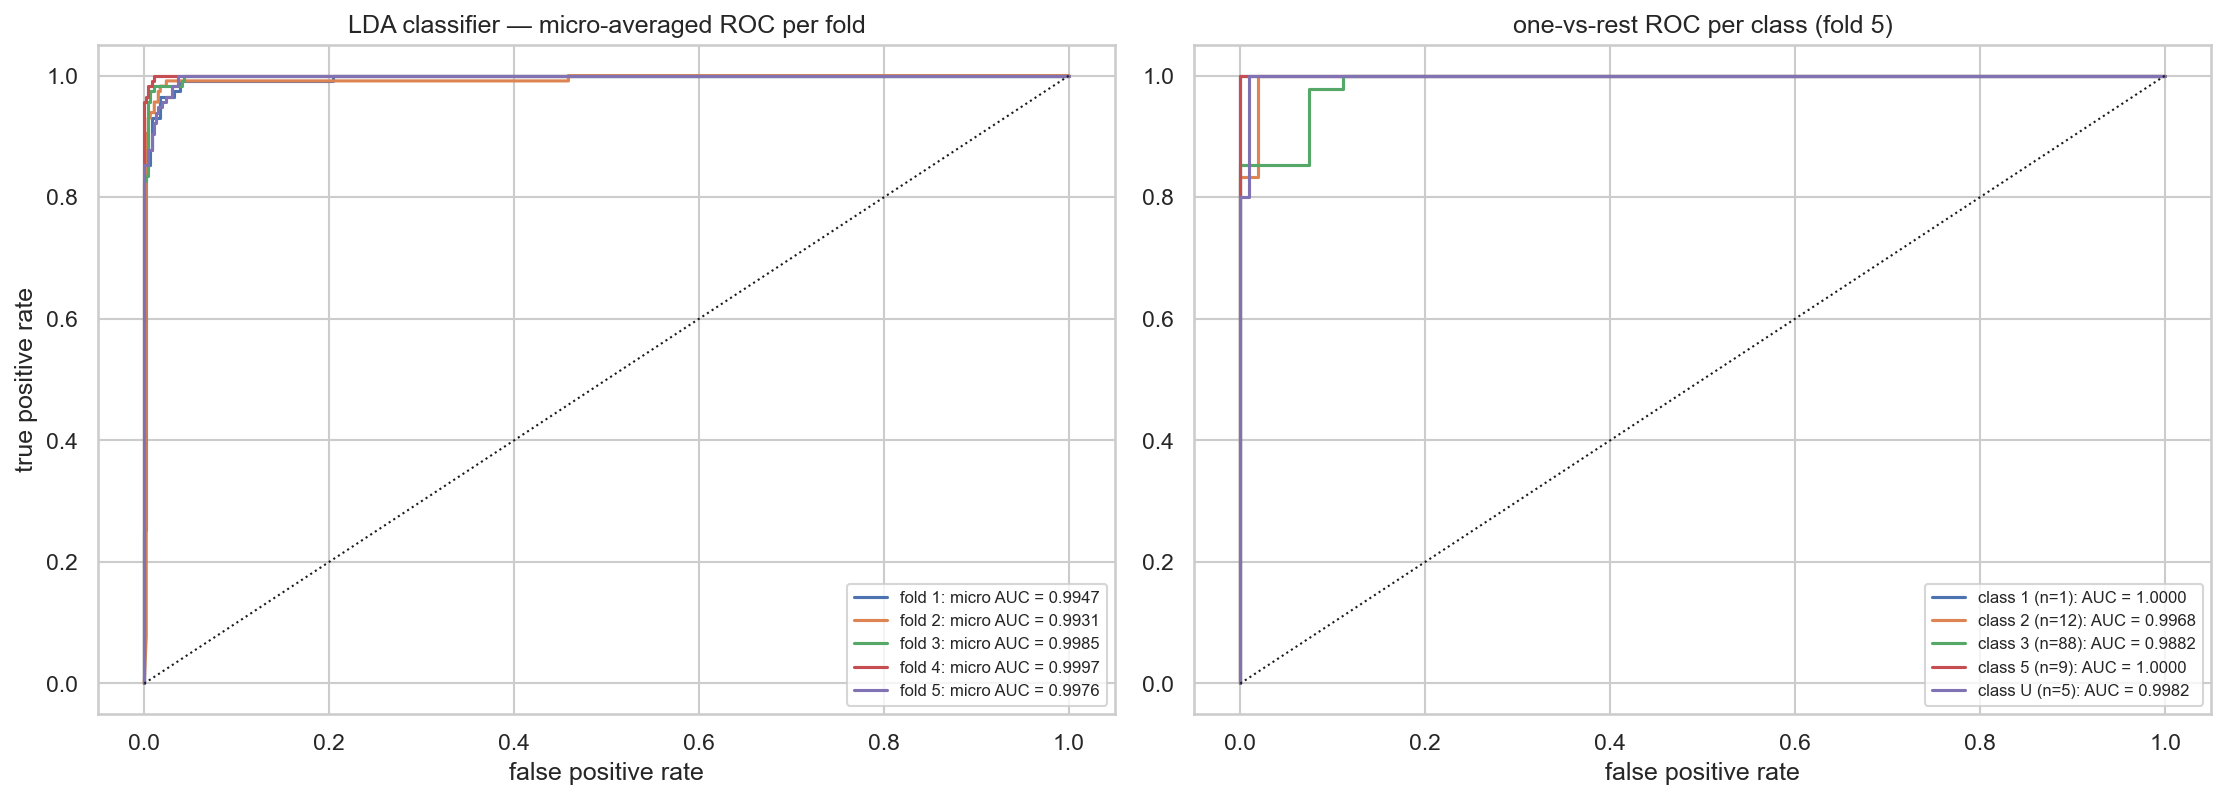
\includegraphics[width=\linewidth]{figures/q2_roc.png}
\caption{Micro-averaged ROC per fold (left) and one-vs-rest ROC per class on fold 5 (right).}
\end{figure}
Class 5 is ranked perfectly in every fold (AUC 1.0), for the reason given above. The weakest class is U (mean AUC 0.971; 0.866 in fold 1):
it is a small, heterogeneous ``unclassified'' group that shares feature values with class 3. The AUCs are much higher than the accuracies,
because ranking a sample correctly is easier than placing it on the right side of a single threshold. For example, the probabilities usually put class-U samples
above most class-3 ones, but not always above the decision point.

\end{document}
